\chapter{Introduction}

Proteins are essential to and found in all extant life on Earth.
They function as enzymes, performing factory-like transformations of chemicals,
provide structural support and function as machine that can move organisms,
are integral to transportation and communication within and between cells,
and are the basis of the ability of our immune systems to detect antigens.
In fact, proteins are so important for the function of life that their blueprints are written in our DNA\cite{avery_studies_1944} using a near-universal encoding\cite{crick_origin_1968,hinegardner_rationale_1963},
providing evidence for Darwin's theory that all life on Earth shares common ancestry\cite{darwin_origin_1859}.

Understanding how proteins work can be undertaken using a variety of strategies, including genetic analysis \cite{lander_initial_2001}, but one of the most informative has been to determine the structure of proteins, as knowing what a machine looks like provides insight into its functionality.
We have been able to determine the structures of proteins at a high resolution since the first published crystal structures of myoglobin and hemoglobin(\cite{kendrew_three-dimensional_1958,perutz_structure_1960}.
Still, there are many more known protein sequences in the universe of life than exist known structures in available databases of experimentally determined structures (88,032,926 unique sequences vs. 123,153 known structures, as of Aug. 12, 2017 \cite{berman_protein_2000,noauthor_uniprot:_2017}).

Obtaining models of structures where no experimental data exists would help provide insight into the vast space of unknown protein functionality.
In these cases, we can turn to the power of computation to help determine unknown structures.
Developing computational protocols for protein structure provides a few great advantage, including the fact that a method capable of accurately predicting protein structure can also be adapted to design entirely new protein functionalities.
This ability to design proteins enables the creation of protein therapeutics potentially capable of treating currently untreatable diseases, as well as enzymes that could be able to make chemicals and fuels in a more environmentally friendly fashion.

The value of computational methods for protein structure prediction goes beyond their potential applications in design.
By attempting to create a framework in which we can accurately represent, sample, and score and compare models of protein structures, we gain insight into the inner workings of the biophysics that underlie the functionality of proteins in all life.

\section{Computational protein structure prediction and design}

\begin{wrapfigure}{L}{0.5\textwidth}
  \centering
  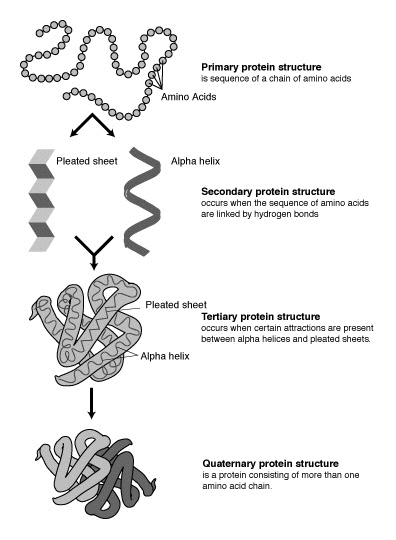
\includegraphics[width=0.48\textwidth,keepaspectratio]{figures/protein-structure.png}
  \caption[Protein sequence/structure]{Knowledge of the primary amino acid sequence is a common input for computational structure prediction programs, which then can produce possible models of the protein's secondary, tertiary, and quaternary structure. Figure produced by: U.S. National Institutes of Health (public domain).}
  \label{fig:protein-structure}
  \vspace{-12pt}
\end{wrapfigure}

Protein structure prediction can operate on the ``primary'', ``secondary'', ``tertiary'', or ``quaternary'' levels (\cref{fig:protein-structure}).
While modern protein secondary structure prediction methods can achieve relatively high accuracy (of about 80\%\cite{pirovano_protein_2009}), protein structure prediction of more detailed models remains a major challenge.

The difficulty of computational protein structure prediction can be thought of as three complementary challenges: the ``sampling'' problem, the ``scoring'' problem, and the question of ``representation''.

\paragraph{Representation}
Choosing a manner in which to represent protein structures within the overall computational framework that fits the desired application is an oft-overlooked, but essential step in modeling.
For example, software that attempted to internally represent proteins as a collection of subatomic components such as proteins, neutrons, or even quarks, would be a far more detailed representation than is required for simulating biologically relevant processes such as protein-protein interactions.
Computational time would be wasted simulating the interactions of subatomic particles if the desired output can be obtained by simulating the system at a coarser level of detail.
On the other hand, representing proteins as individual spheres that interact and bounce off each other like billiard balls would be too simplistic for many applications, and would not be able to simulate at the level of detail required for predicting the specificity and strength of binding interactions.
In the end, a balance must be struck, and full-atom representations of protein structures are now commonly used in modeling.

\paragraph{Scoring}
Scoring refers to the ability of a prediction/design method to successfully rank and sort generated models of protein (in whichever representation they are generated) in terms of stability or other desired biophysical attributes.
Again, as with representation, an appropriately detailed score function should be chosen to fit the problem at hand.
Score functions used in protein modeling and design have taken a variety of approaches, including modeling atomic interactions with solvent both explicitly\cite{duan_pointcharge_2003,brooks_charmm:_2009} or implicitly\cite{lazaridis_effective_1999}, repulsive and attractive terms\cite{lennard-jones_determination_1924}, and knowledge-based terms calibrated based on the propensity of protein substructures to occupy various states\cite{rohl_protein_2004}.
If a score function is to be used in protein design, it must be fast enough to evaluate the many potential combinations and permutations of amino acids that could come together to form the entire modeled protein.

\paragraph{Sampling}
Many, many structural models can represent a protein sequence for even the simplest representations of protein structure \cite{levinthal_how_1969,karplus_levinthal_1997}.
The sampling problem refers to the difficulty of generating protein structural models out of this near-infinite universe of potential states.
As only a finite number of models can be scored, decoy models must be generated efficiently.
Sampling methods that have proven to be effective include modifying a known protein structure for new activity\cite{jiang_novo_2008,siegel_computational_2010}, design of a protein backbone to fit a desired topology\cite{kuhlman_design_2003}, defined ``moves'' that are likely to jump between stable structures\cite{davis_backrub_2006,mandell_sub-angstrom_2009,friedland_simple_2008}, and a divide-and-conquer approach that breaks proteins into ``fragments'' that can be sampled individually \cite{simons_assembly_1997}.

\section{Ways forward to improve computational protein modeling}
Although proteins tend to ``fold'' into energy minima centered on the globally most stable conformation\cite{dill_levinthal_1997}, life takes place at non-frozen, biological temperatures.
In cells, proteins are dynamic and sample an ensemble of conformations centered around free-energy minima\cite{henzler-wildman_dynamic_2007}.
Protein modeling and design software might therefore obtain improved predictions from representing proteins more complexly, allowing for conformational flexibility.

In my graduate research, I set out to develop and test sampling and representation methods that allowed for more realistic models of proteins, enabling design of new protein functions and predictions of protein structures that could better explain the inner functionality of biological systems.
I have developed these methods within the Rosetta macromolecular modeling suite, which is developed by researchers around the world, allowing access to improved score function and sampling methods as they are developed by others.

Since the problem of scoring is inextricably linked to the problem of sampling, I needed to rigorously test the performance of new score functions on rationally created benchmark datasets, providing a foundation of known performance to build up to these more complex representations (\cref{chapter:web-benchmark}).
I then developed a method capable of predicting the change in strength of protein-protein interactions after mutation (\cref{chapter:flex-ddG}) that utilizes ensemble-based representations of protein structure that more accurately.
As I, in collaboration with my cohort of iPQB graduate students, have already shown the ability of Rosetta to to provide insight into the mechanisms of how changes in strength in protein-protein interactions affect fitness in yeast \cite{mavor_determination_2016,mavor_extending_2017}, I hope and expect that these developments in computational protein modeling methodology will continue to prove useful in the future in biological applications